\documentclass[conference]{IEEEtran}
\usepackage{cite}
\usepackage{amsmath}
\usepackage{amsfonts}
\usepackage{amssymb}

%--------package image---------------------------------------------------------
\usepackage{graphicx}
\usepackage{subfig}
\graphicspath{{./imgs/}}
\renewcommand{\figurename}{Fig.}

%-------package tikz-----------------------------------------------------------
\usepackage{tikz,fp,ifthen,fullpage}
\usepackage{pgfmath}
\usetikzlibrary{backgrounds}
\usetikzlibrary{decorations.pathmorphing,backgrounds,fit,calc,through,
decorations.markings}
\usetikzlibrary{arrows}
\usetikzlibrary{shapes,decorations,shadows}
\usetikzlibrary{fadings}
\usetikzlibrary{patterns}
\usetikzlibrary{mindmap}
\usetikzlibrary{decorations.text}
\usetikzlibrary{decorations.shapes}
\usepackage{pgfplots}
\pgfplotsset{compat=1.13}
%--------------------------Document--------------------------------------------
\begin{document}
%Here goes the title
	\title{Enter your Paper Title Here}
%Authors List
	\author
	{\IEEEauthorblockN{Francesco Argentieri}
		\IEEEauthorblockA{ID 183892\\
		Email: francesco.argentieri@studenti.unitn.it}
		%\and
		%\IEEEauthorblockN{Author 2}
		%\IEEEauthorblockA{University\\
		%Location\\
		%Email: }
	}
	\maketitle
%Main body starts
	\begin{abstract}
		Abstract goes here
	\end{abstract}
% define keyword
	\begin {IEEEkeywords}
		IoT, Ontology, Semantics,  SSN, OWL, OBOE, OpenIoT, SWEET, SUMO
	\end{IEEEkeywords}
	%Introduction
	\section{Introduction}
\label{sec:intro}
In this era, a large amount of structured and unstructured data became available.
\textbf{Machine Learning} (\textbf{ML}) has evolved as a branch of artificial
intelligence: it envisages the development of self-learning algorithms, which are
capable of acquiring knowledge from data with the aim of making predictions.
Instead of requiring a human presence who manually enact the rules and
build models for the analysis of large amounts of data, machine learning offers
a more efficient alternative to capture the knowledge in the data. Machine learning
aims to gradually improve the performance of forecasting models and
to make data driven decisions.
In this section we will examine the three different types of machine learning:
\emph{supervised learning}, \emph{unsupervised learning} and
\emph{reinforcement learning}.
Where we will show the fundamental differences between these types of
learning.\cite{raschka2016machine}
%
\subsection{Supervised learning}
\label{subsec:supervised-learnig}
The main purpose of supervised learning is to derive a model from 
training data, which allows us to make predictions for data that are not
available or future.
Here, the term ``supervision" refers to the fact that the output signal labels of the
sample sets are already known.
A supervised learning task, which is based on discrete class labels, is also called a
classification task.
Another supervised learning subcategory is regression, whose resulting
signal is a continuous value.
Classification is a sub-category of supervised learning, which has the goal to
provide class category labels for new instances, based on observations made in
the past.
These labels are discrete, unordered values ​​that can be considered as
belonging to a group of instances.
However, the set of class labels does not necessarily have to be a binary
nature.
The predictive model identified by a supervised learning algorithm can consider
each class label that is present in the learning dataset of a new instance, which
is not labelled.\\
A typical example of \emph{multi-class classification} is the recognition of
hand-written text.\cite{raschka2016machine}
%
\begin{figure}[!h]
\centering
%\draw [help lines] (0,0) grid (8,8);
\resizebox{\linewidth}{!}{\begin{tikzpicture}[auto,>=latex']
%\draw [help lines] (0,0) grid (8,8);
\tikzset{
	boxA/.style={
  		rectangle,
  		inner sep=0pt,
  		text width=25mm,
  		align=center,
  		draw=black,
  		fill=airforceblue,
  		minimum height = 10mm
  	},
  	boxB/.style={
  		rectangle,
  		inner sep=0pt,
  		text width=25mm,
  		align=center,
  		draw=black,
  		fill=amber,
  		minimum height = 10mm
  	},
  	boxB1/.style={
  		rectangle,
  		inner sep=0pt,
  		text width=25mm,
  		align=center,
  		draw=black,
  		fill=amber!30,
  		minimum height = 10mm
  	},
  	boxC/.style={
  		rectangle,
  		inner sep=0pt,
  		text width=25mm,
  		align=center,
  		draw=black,
  		fill=light-gray,
  		minimum height = 10mm
  	},
  }

\node (a) [boxC, align=center] at (1,1) {New data};
\node (b) [boxC, align=center] at (5,1) {Predicitve\\ model};
\node (c) [boxC, align=center] at (9,1) {Prediction};
\node (d) [boxA, align=center] at (5,3) {Alogrithm\\ DNN};
\node (e) [boxB, align=center] at (5,5) {Dataset};
\node (e1) [boxB1, align=center] at (6,5.85) {Label};
\draw [->] (a) -- (b);
\draw [->] (b) -- (c);
\draw [->] (d) -- (b); 
\draw [->] (e) -- (d); 
\end{tikzpicture}}
\caption{supervised learning scheme} 
\label{fig:supervised-learning-scheme}
\end{figure}
%
\subsection{Reinforcement learnig}
\label{subsec:reinforcement-learnig}
Another type of machine learning is reinforcement learning.
Here, the goal is to develop a system (\emph{agent}) for people to improve
their performance. In order to do so, that system is based on interactions with 
the environment.
Since information relating to the current state of the environment
include also a \emph{reward} signal, we can consider strengthening
learning as an example of supervised learning.
However, this feedback is not the correct label or the
true value of truth, but it represents the quality of the measurement of the 
performance measured by the reward function.
Through interaction with the environment, an agent can then use reinforcement
learning to learn a series of actions, which maximize this reward through a
trial-and-error exploratory approach or deliberative planning.\cite{raschka2016machine}
%
\begin{figure}[!h]
\centering
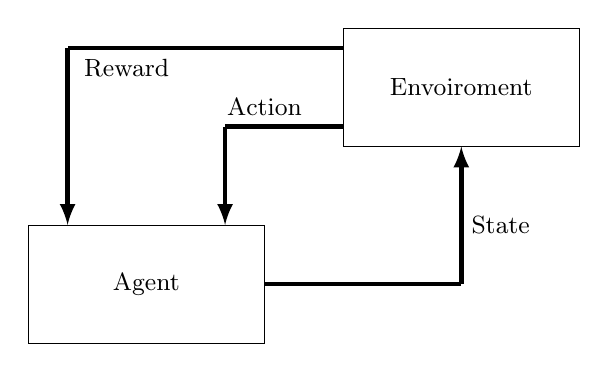
\begin{tikzpicture}[>=latex]
 %\draw [help lines] (0,0) grid [step=0.5] (8,4);
 \draw (0.5,0) rectangle ++(3cm, 1.5cm);
 \draw (4.5,2.5) rectangle ++(3cm,1.5cm);
 %\node [draw] (1.5,2) {Agent};
 \coordinate [label={[font=\small]center:Agent}] (A) at (2,0.75);
 \coordinate [label={[font=\small]center:Envoiroment}] (E) at (6,3.25);
 \draw [-, ultra thick] (3.5,0.75) -- (6,0.75);
 \draw [->, ultra thick] (6,.75) -- (6,2.5);
 \coordinate [label={[font=\small]center:State}] (S) at (6.5,1.5);
 %
 \draw [-, ultra thick] (4.5,2.75) -- (3,2.75);
 \draw [->, ultra thick] (3,2.75) -- (3,1.5);
 \coordinate [label={[font=\small]center:Action}] (T) at (3.5,3);
 %
 \draw [-, ultra thick] (4.5,3.75) -- (1,3.75);
 \draw [->, ultra thick] (1,3.75) -- (1,1.5);
 \coordinate [label={[font=\small]center:Reward}] (R) at (1.75,3.5);
\end{tikzpicture} 
\caption{reinforcement learning scheme} 
\label{fig:reinforcement-learning-scheme}
\end{figure}
%
\subsection{Unsupervised learning}
\label{subsec:unsupervised-learning}
In supervised learning, we know in advance the correct answer when we describe
our model, while in reinforcement learning we define a measure, or reward, for
the specific actions performed by the agent.
In unsupervised learning, on the other hand, we are dealing with unlabelled data
or data from the unknown structure.
Using unsupervised learning techniques, we are able to observe the structure of
our data, to extract meaningful information from them without being able to
rely on the guide nor a variable known relative result, nor a reward function.
Clustering is an exploratory technique of data analysis that allows us to
organize a series of information within meaningful groups (\emph{cluster})
without having any previous knowledge of memberships in such groups.
Each cluster that can be derived during the analysis defines a group of objects
that share a certain degree of similarity, but which are more dissimilar than
the objects present in the other clusters, which is why clustering is sometimes
called \emph{``unsupervised classification"}.
Clustering is an excellent technique for structuring information to identify
meaningful relationships in the data.\cite{raschka2016machine}
%
\begin{figure}[!h]
\centering
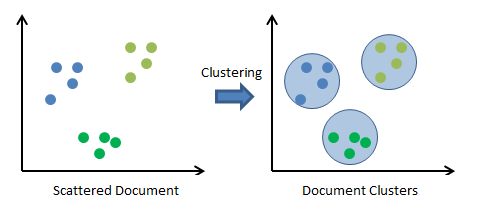
\includegraphics[width=\linewidth]{cluster}
\caption{example of clustering}
\label{fig:unsupervised-learning-scheme}
\end{figure}
%
%\subsection{Prerequisites}
%\label{subsec:rerequisites}
%The code requires Python 3.5.2 or higher (version 3.7 is not supported) to be
%installed on a MacOS, Linux or Windows system.
%Referring to essential libraries dedicated to the scientific group, including
%SciPy, NumPy, scikit-learn, matplolib and pandas.
%We will add the TensorFlow-gpu library for efficient training of neuronal
%networks on GPU units.

	\section{Deep learning}
\label{sec:deeplearning}
%
Deep learning lies at the heart of the most advanced machine learning solutions,
such as those that have learned to recognize items and images, determine the
sentiment of text, and drive vehicles. 
These neural networks are complex and can be challenging to build, but Keras 
removes much of the effort.
Keras acts as an API\footnote{application programming interface (API) is a set 
of subroutine definitions, communication protocols, and tools for building 
software. In general terms, it is a set of clearly defined methods of 
communication among various components. 
A good API makes it easier to develop a computer program by providing all the 
building blocks, which are then put together by the programmer.\cite{API}}, 
letting us quickly create a network that might take hours or days to hand code 
in Python or other languages.
%
\subsection{Introducing Keras}
\label{sec:introduction_keras}
Let's use the definition from the documentation at keras.io.
Keras is a high-level neural network API, written in Python and capable of
running on top of TensorFlow, CNTK or Theano.\cite{chollet2015keras}
That is, it lets us build neural networks easier by providing us with a
high-level set of constructs.
These constructs handle much of the plumbing involving in wring up neural
networks and thus reduce programming errors.
Also, as an API, it provides an interface that we can develop against and a
detailed description of what happens when we invoke various objects and methods.
Keras is Python centric in its code and is implemented as a Python library.
It is imported and used just like any other Python library you might be familiar
with, so the learning curve is minimal.
Finally, Keras runs on top of \emph{TensorFlow}, \emph{CNTK}, or \emph{Theano}.
These are three of the most widely used libraries for performing work with
neural networks.
Keras calls these libraries to perform the actual execution of operations that
create, populate, train, and evaluate the neural networks we specify in Keras.
Keras utilizes either TensorFlow, CNTK, or Theano as the 
\emph{backend}\footnote{In software engineering, the terms front end and back 
end refer to the separation of concerns between the presentation layer (front 
end), and the data access layer (back end) of a piece of software, or the 
physical infrastructure or hardware. In the client--server model, the client 
is usually considered the front end and the server is usually considered the 
back end, even when some presentation work is actually done on the server.
\cite{backend}}.
Keras itself does not create or execute the neural network.
Rather, Keras defines an API we code against. 
In our code we invoke Keras methods and pass the appropriate parameters.
Keras evaluates these for correctness and constructs whatever objects are
required.
Keras then calls the appropriate backend methods to do the actual neural 
network operations, such as defining structures, training the neural network 
model, and evaluating the trained model. Any result from these operations are 
returned by the backend to Keras, which processes them and returns to our code 
the appropriate results.
%
\begin{figure}[!h]
\centering
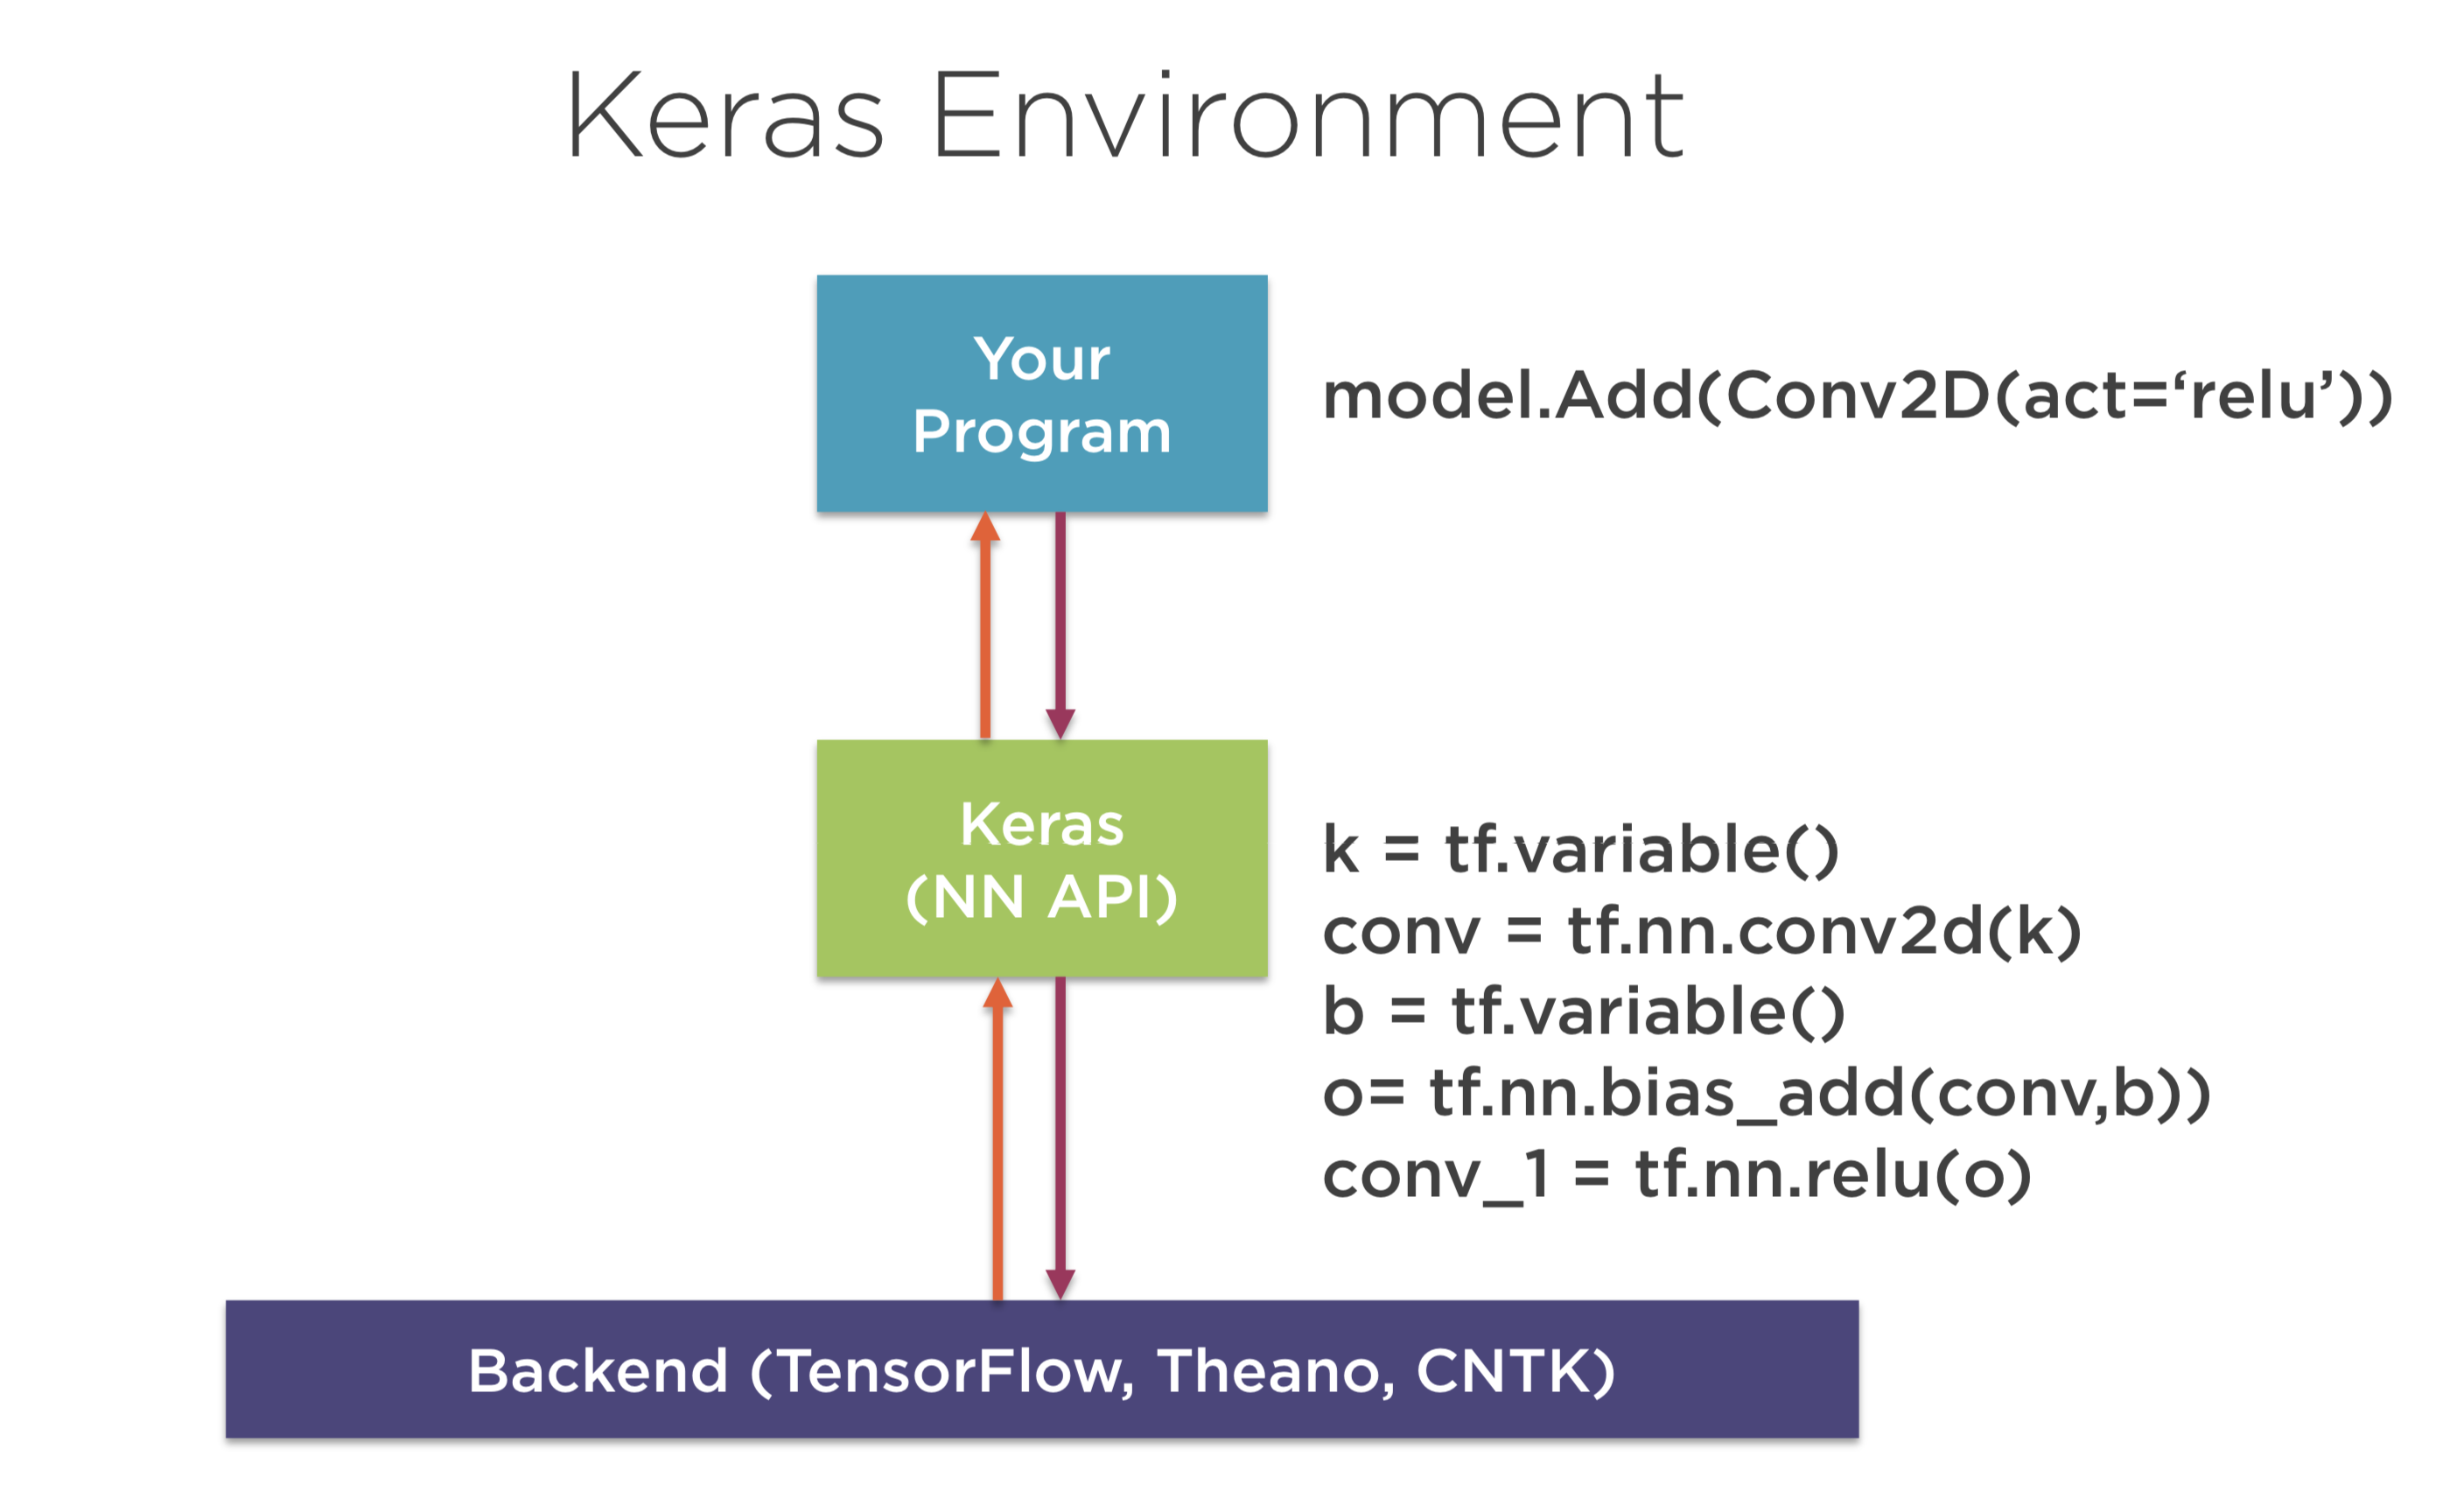
\includegraphics[width=\linewidth]{enviroment}
\caption{Keras enviroment}
\label{fig:nn_layer}
\end{figure}
%
\section{Neural Networks}
\label{sec:neuralnetwork}
%
The neural network, in figure \ref{fig:nn_layer}, where on the 
left we have the input layer, which feeds data into the network.
This data could be values from a data table, images from a camera, sounds from a
recording, or output from a sensor.
The input layer does not change the data, it simply passes it for processing by
the remaining layers. The data from the input layer is passed to another layer
of neurons.
These layers can be of different types with the different layer types performing
different transformations on the data as required by our solution. In a simple
network, the input layer can be directly connected to an output layer of neurons,
which provide the final outputs.
%
\begin{figure}[!h]
\centering
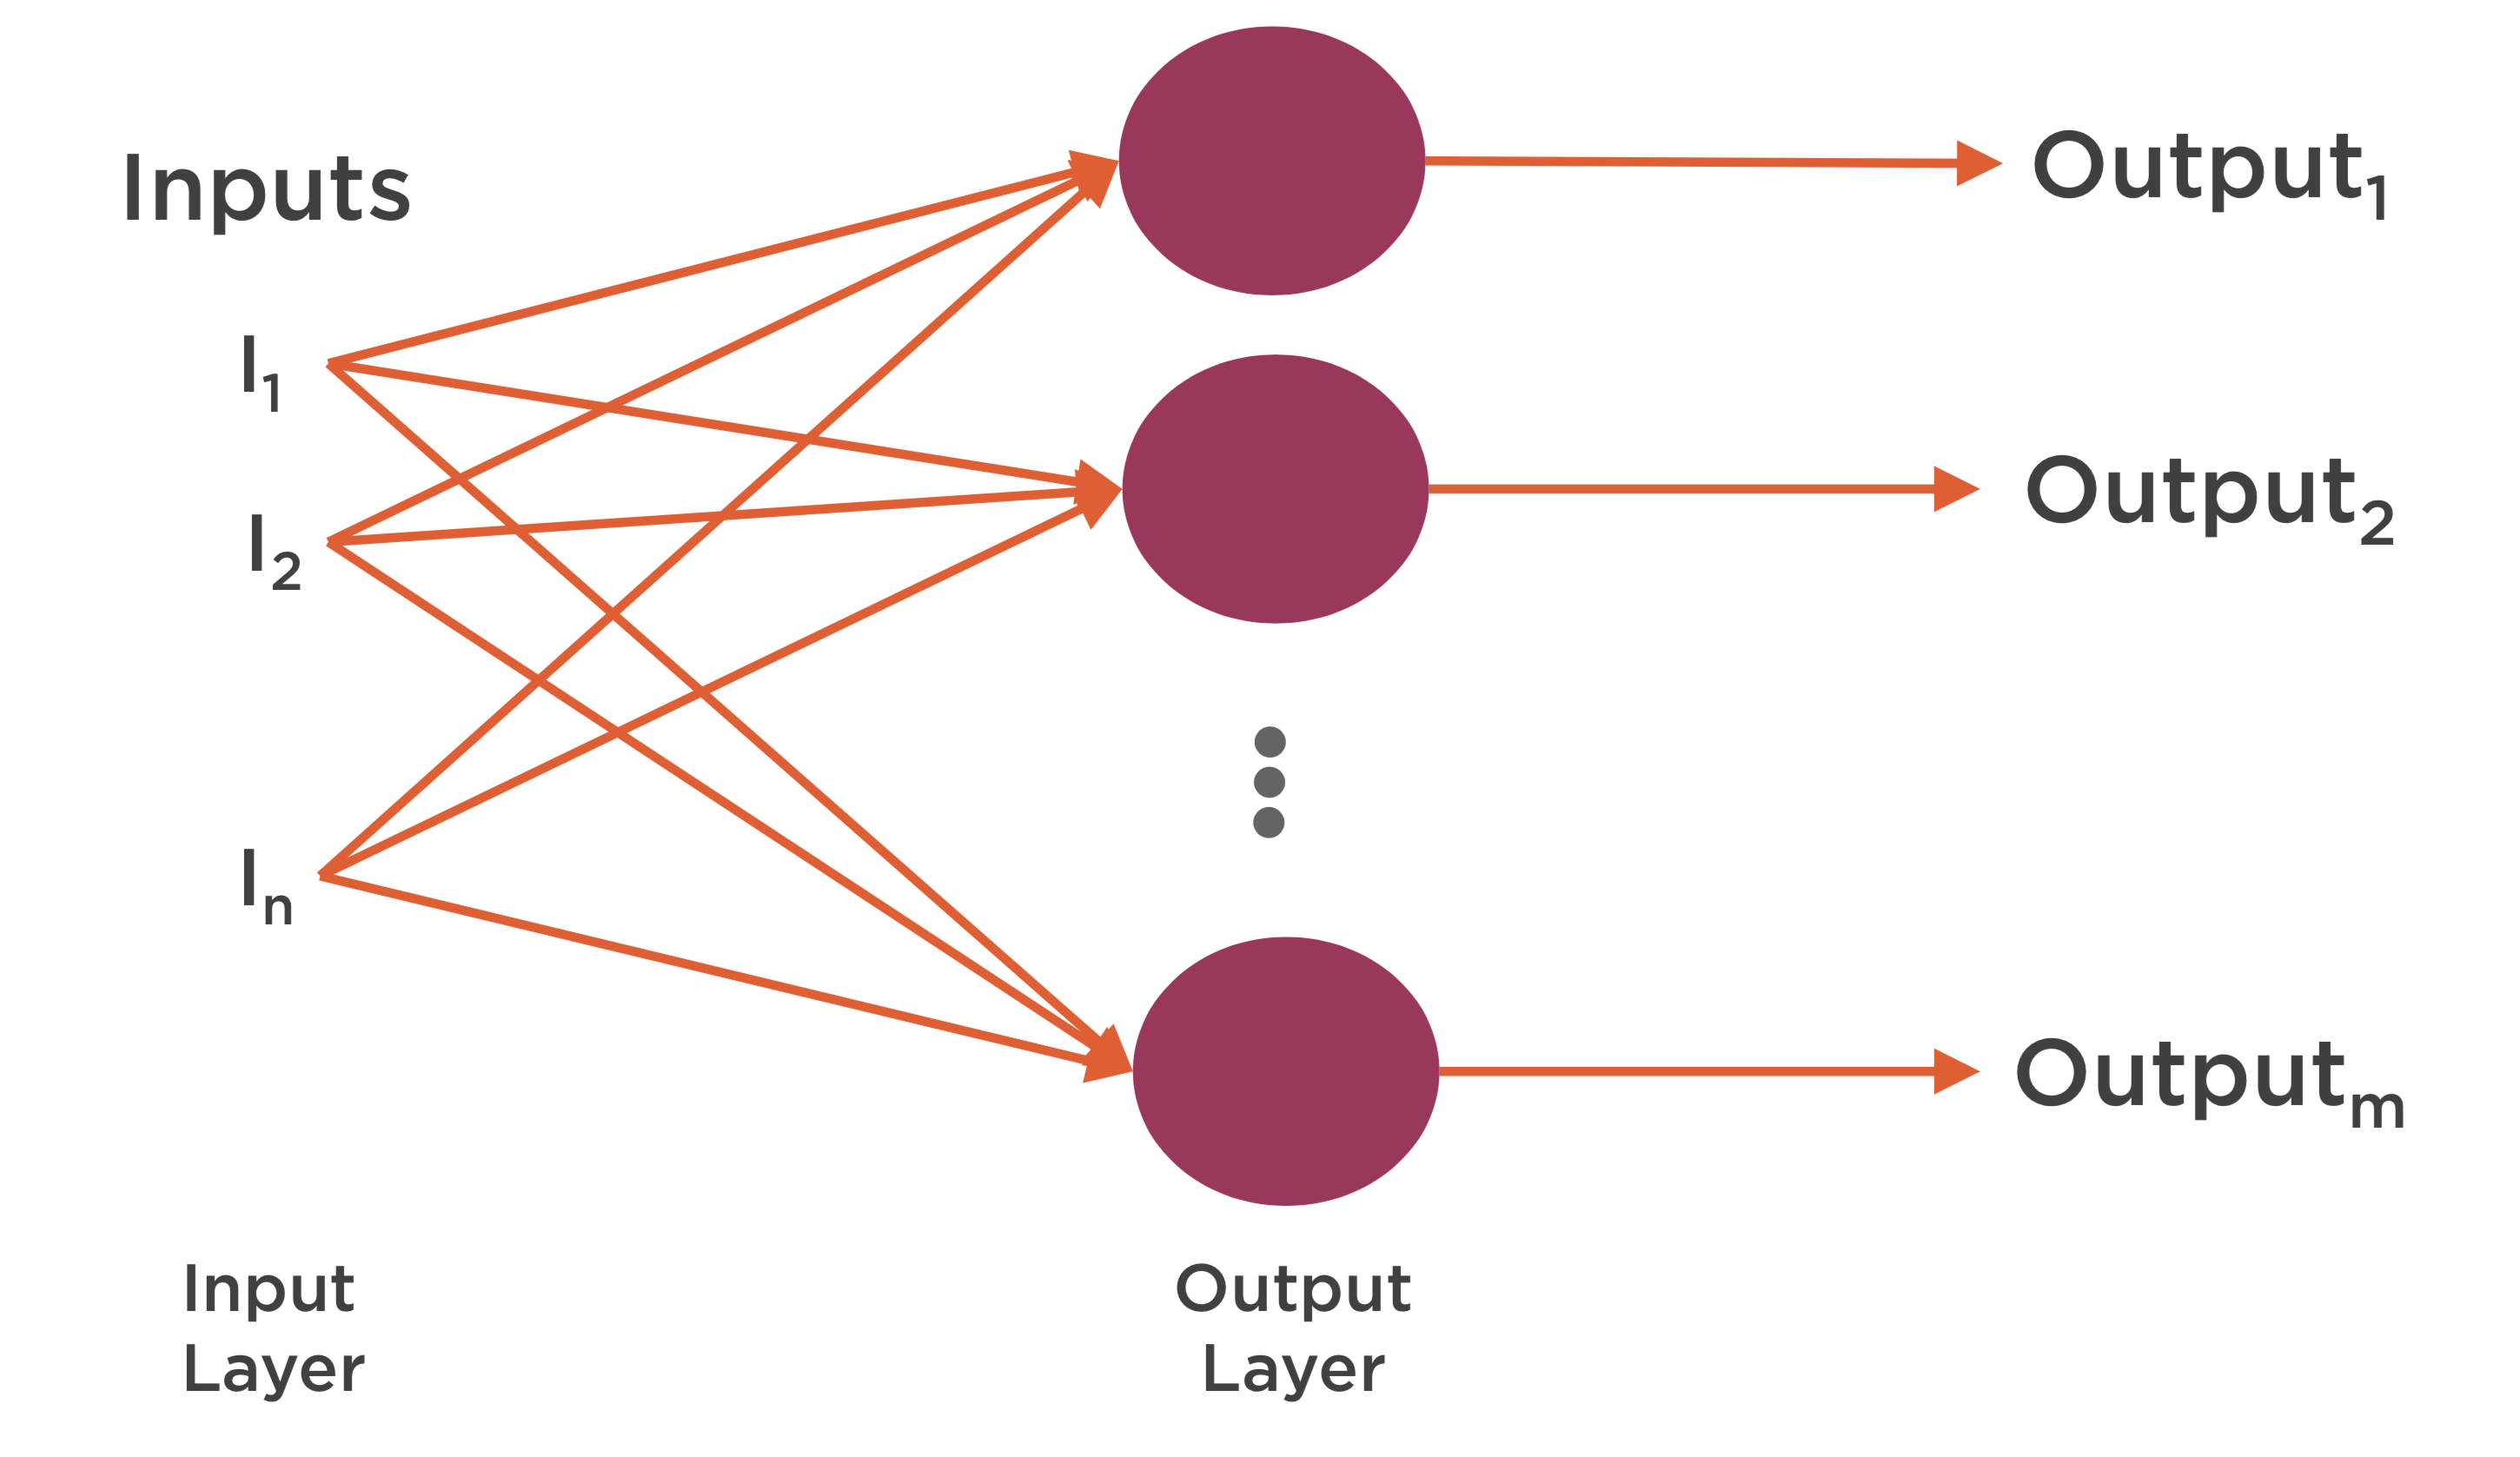
\includegraphics[width=\linewidth]{neuralnetwork}
\caption{Neural networks layers}
\label{fig:nn_layer}
\end{figure}
%
But in most networks, the input layer is connected to hidden layers.
Hidden layers are defined as not being input or output layers, and therefore,
are hidden to the code that's using the neural network.
The network can have many hidden layers and if there are two or more hidden
layers we call the network a deep neural network.
%
\begin{figure}[!h]
\centering
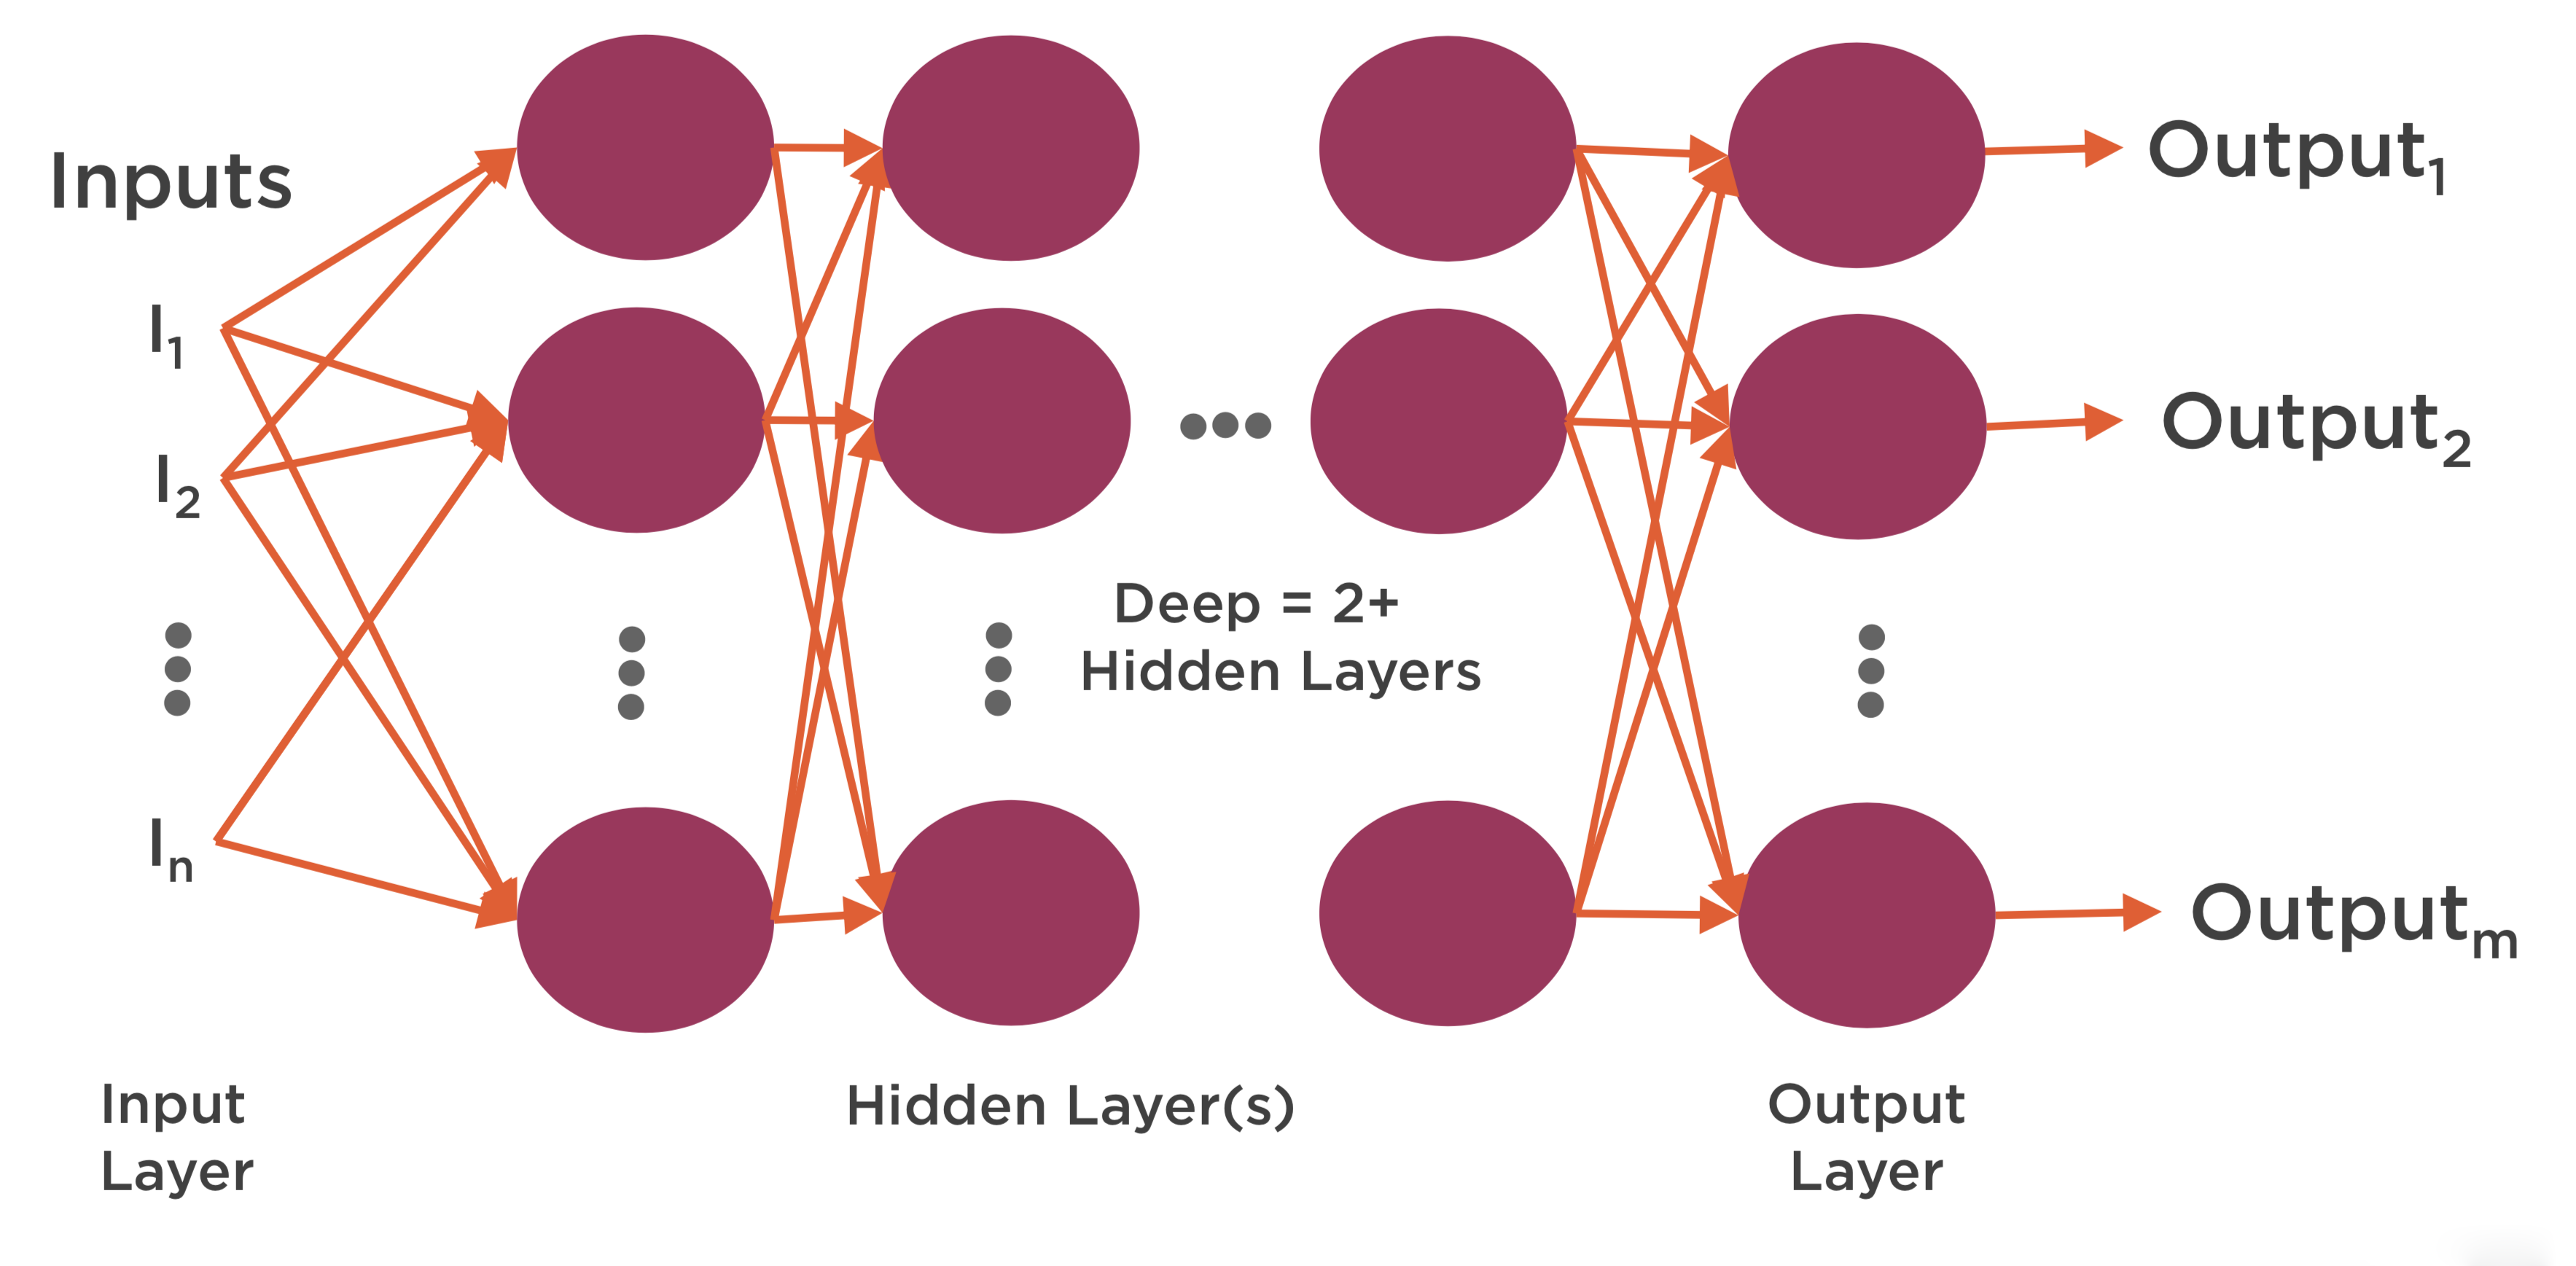
\includegraphics[width=\linewidth]{deep_nn}
\caption{Deep neural networks layers}
\label{fig:deepnn}
\end{figure}
%
In this learning process we adjust the structures of our neurons.
To understand this, let's look at a single neuron. Here we see the inputs and
outputs we showed in the network diagram, with the inputs going in and the
outputs going out.
However, what is not showing in this diagram is how the neurons work internally.
To do that, we need to open the neuron so we can see how it is constructed.
As we see, the neuron is performing a simple mathematics summing of weights times
the input value and adding a bias.
The product of these operations is passed through a non-linear activation function.
And the output of the activation function is the output of the neuron.
A key feature of the neural network is the ability to use the input data to
train the weights and biases so the signal passed out of the neuron changes
based on the input data. To do this training, we expose the network to data.
With each set of data, an algorithm is used to adjust the weights and bias to
minimize the error the network has in predicting the data's values.
This is done through processes called forward propagation and back propagation.
And when these processes are complete, the network is said to be trained, and
the weights and biases of all the neurons have been adjusted to give the best
results on the training data. So to summarize, the neural network consists of
three layer types, input, hidden, and output. 
By passing training data through the network, the network of neurons is 
trained to give results with the least error.
This training is done by adjusting weights and biases in the neurons, utilizing
the processes of forward propagation and back propagation, and if there are two
or more hidden layers in the network, we say it's a deep neural network.

	\section{Building Convolutional Neural Network with Keras}
\label{sec:buildcnn}
%
As we discussed in section (\ref{subsec:introduction_keras}), Keras 
has a series of layers that were specifically created to support convolutional 
neural networks.
By definition, a fully connected layer connects every neuron in the layer and 
at the first layer it's connected to all the inputs. 
And all these connections create a problem known as the curse of 
dimensionality. 
That is, the more neurons and connections we have, the more weights we must 
train. 
This issue appears often, it is one of reasons why deep neural networks can 
take a long time to learn. 
To understand this issue a bit more, let's consider the case of working with 
images. 
Assume that we have an 8 megapixel image and that we want to learn 
something from this image. 
To do that, we construct a network with a dense layer. 
Since every pixel in the image can contain unique data, they each contribute 
uniquely to determining the logic resulting from analysing the image. 
Therefore we need to connect each pixel to each neuron in our first layer. 
Let's say that we have 1000 neurons in the first dense layer.
We have to connect the data from each pixel to each neuron so we end up with 
1000 neurons connected to 8 million pixel values, with each connection having 
its own weight that needs to be trained. 
That works out to 8 billion weights we have to train. 
And with most images it's even more. In a color image, each pixel has three 
colors. 
One for red, green, and blue channels of the image. 
So there are actually 24 billion weights to train.
Solving this explosion in the number of weights we have to train is one of the 
key reasons convolutional neural networks were developed. 
%
\subsection{How works CNNs}
\label{ssec:cnnworks}
%
Convolutional neural network address our two concerns of working with image 
type data namely, many weights to train and being able to detect objects based 
on their general appearance rather than precisely matching an image. 
A lot of research has been performed when working with images and has 
resulted in subtle layers that you find in almost all convolutional neural 
networks. 
And these are the convolution layers you find in Keras. 
To understand the function of these layers, let's go over the structure of a 
convolutional neural network, which classifies objects and images.
%
Let's walk through this diagram so we can get an overview of how convolutional 
neural networks work and how we implement them using Keras. 
We see the image data is passed through the convolutional layer, then through 
a non-linear ReLU activation and then to a pool layer. 
And then to a second convolution with ReLU layer and a second pool layer. 
Finally, to a fully connected layer and then to a second fully connected 
layer for classification. 
So we can divide our convolutional neural network into four operations. 
Convolution, non-linearity, you see via ReLU, pooling, and classification. 
You will find these four operations in almost all convolutional neural networks. 
Let's look at each operation in detail so we understand how to set parameters 
and pass data when we construct our convolutional neural network in Keras.
Convolutional neural networks are the current state-of-art architecture for
image classification. They are used in practice today in facial recognition, self
driving cars, and detecting whether an object is a hot-dog.
%
\subsection{Convolution}
\label{ssec:convolution}
%
A convolution consists of a kernel, shows in figure \ref{fig:convolution}, 
(green square above), also called filter,
that is applied in a sliding window fashion to extract features from the input.
This filter is shifted after each operation across the input by an amount called
strides. At each operation, a matrix multiply of the kernel and current region
of input is calculated. Filters can be stacked to create high-dimensional
representations of the input.
%
\begin{figure}[!h]
\centering
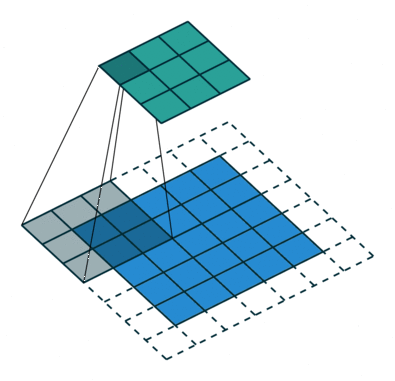
\includegraphics[width=\linewidth]{conv_arithmetic}
\caption{Convolution operation to extract features from the input}
\label{fig:convolution}
\end{figure}
%
There are two ways of handling differing filter size and input size, namely
same padding and valid padding.
Same padding will pad the input border with zeros (as seen above) to ensure the
input width and height are preserved. Valid padding does not pad.
Typically, you will want to use same padding or you will rapidly reduce the
dimensionality of your input.
Finally, an activation function (typically a ReLU\footnote{In the context of 
artificial neural networks, the rectifier is an activation function defined as 
the positive part of its argument:\\ \(f(x) = x^{+} = \text{max}(0,x)\)}), 
represented in figure \ref{fig:relu}, is applied to give the convolution non-linearity.
ReLU’s are a bit different from other activation functions, such as sigmoid or
tanh, as ReLUs are one-sided.
This one-sided property allows the network to create sparse representation
(zero value for hidden units), increasing computational efficiency.
%
\begin{figure}[htb]
\centering
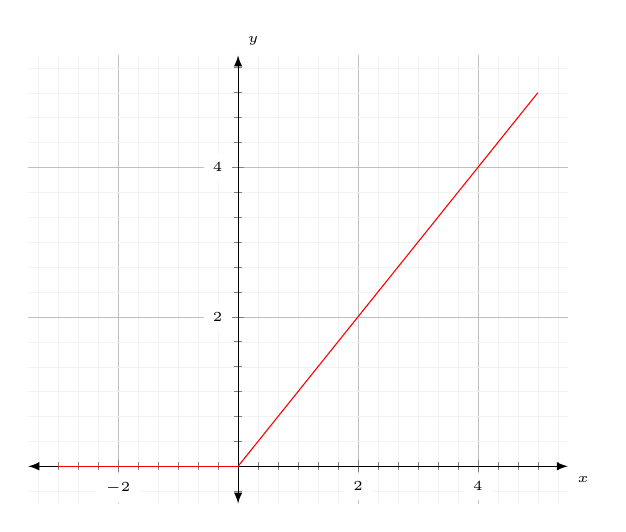
\begin{tikzpicture}
    \begin{axis}[
        domain=-3:5,
        grid=both,
    	grid style={line width=.1pt, draw=gray!10},
    	major grid style={line width=.2pt,draw=gray!50},
    	axis lines=middle,
    	minor tick num=5,
    	enlargelimits={abs=0.5},
    	axis line style={latex-latex},
    	ticklabel style={font=\tiny,fill=white},
    	xlabel style={at={(ticklabel* cs:1)},anchor=north west},
    	ylabel style={at={(ticklabel* cs:1)},anchor=south west},
    	xlabel={\tiny $x$},
    	ylabel={\tiny $y$}
    ]
        \addplot+[mark=none,red,domain=-3:0] {0};
        \addplot+[mark=none,red,domain=0:5] {x};
    \end{axis}
\end{tikzpicture}
\caption{Rectified linear unit (\textbf{ReLU})\\ \(F(x) = x^{+} = \text{max}(0,x)\)}
\label{fig:relu}
\end{figure}
%
\subsection{Pooling}
\label{ssec:pooling}
Pooling is an operation to reduce dimensionality. 
It applies a function summarizing neighbouring information.
Two common functions are max pooling and average pooling.
By calculating the max of an input region, the output summarizes intensity of
surrounding values.
Pooling layers also have a kernel and padding, and are moved in strides, as 
represented in figure \ref{fig:pooling}.
To calculate the output size of a pooling operation, you can use the formula:
\begin{equation}
 \text{Input Width} - \text{kernel width} + 2 * \text{padding}  / \text{strides} + 1
\end{equation}
%
\begin{figure}[htb]
\centering
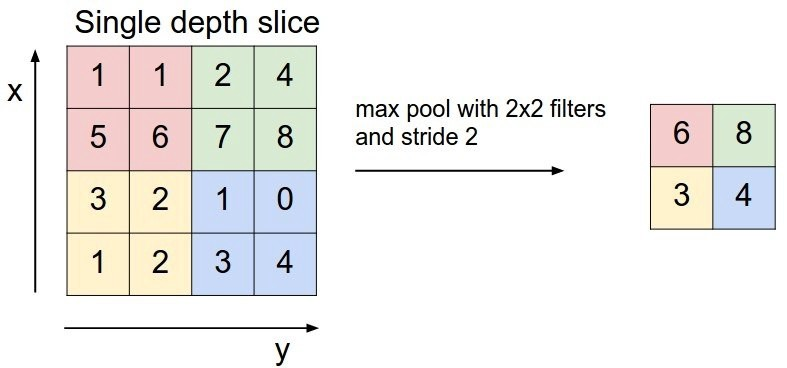
\includegraphics[width=\linewidth]{pooling}
\caption{Max pooling is the application of a moving window across a 2D input 
space, where the maximum value within that window is the output}
\label{fig:pooling}
\end{figure}
%
\subsection{Fully Connected Layer}
\label{ssec:fully_connected}
Fully connected layers you are likely familiar with from neural networks.
Each neuron in the input is connected to each neuron in the output;
fully-connected.
Due to this connectivity, each neuron in the output will be used at most one
time.
%
\begin{equation}
  \sum_{i=1}^{n} \,  x \, \cdot \, W+b
\end{equation}
%
\begin{figure}[htb]
\centering
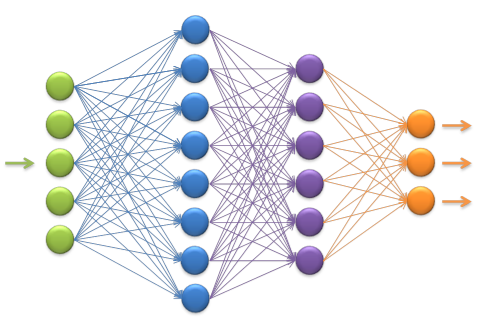
\includegraphics[width=\linewidth]{fully_connected}
\caption{Deep neural networks layers}
\label{fig:fully_connected}
\end{figure}
%
\\\noindent In a CNN, the input is fed from the pooling layer into the fully connected layer.
Depending on the task, a regression or classification algorithm can be applied
to create the desired output, a representative example is shown in figure \ref{fig:fully_connected}.

	%In my last tutorial, you created a complex convolutional neural network from a
%pre-trained inception v3 model.
%In this tutorial, you’ll learn the architecture of a convolutional
%neural network (CNN), how to create a CNN in Tensorflow, and provide predictions
%on labels of images. Finally, you’ll learn how to run the model on a GPU so you
%can spend your time creating better models, not waiting for them to converge.
%
%Overview
%Introduction to CNN’s
%Creating your first CNN and training on CPU
%Training on a GPU
%Prerequisites
%Basic machine learning understanding
%Basic Tensorflow understanding
%AWS account (for gpu)
%
%Convolutional Neural Networks
%Convolutional neural networks are the current state-of-art architecture for
%image classification. They’re used in practice today in facial recognition, self
%driving cars, and detecting whether an object is a hot-dog.
%
%
%Basic Architecture
%The basics of a CNN architecture consist of 3 components. A convolution,
%pooling, and fully connected layer. These components work together to learn a
%dense feature representation of an input.
%
%
%
%Convolution
%
%A convolution consists of a kernel (green square above), also called filter,
%that is applied in a sliding window fashion to extract features from the input.
%This filter is shifted after each operation across the input by an amount called
%strides. At each operation, a matrix multiply of the kernel and current region
%of input is calculated. Filters can be stacked to create high-dimensional
%representations of the input.
%
%
%There are two ways of handling differing filter size and input size, known as
%same padding and valid padding.
%Same padding will pad the input border with zeros (as seen above) to ensure the
%input width and height are preserved. Valid padding does not pad.
%Typically, you’ll want to use same padding or you’ll rapidly reduce the
%dimensionality of your input.
%Finally, an activation function (typically a ReLU) is applied to give the
%convolution non-linearity.
%ReLU’s are a bit different from other activation functions, such as sigmoid or
%tanh, as ReLUs are one-sided.
%This one-sided property allows the network to create sparse representation
%(zero value for hidden units), increasing computational efficiency.
%
%Pooling
%Pooling is an operation to reduce dimensionality. It applies a function
%summarizing neighboring information.
%Two common functions are max pooling and average pooling.
%By calculating the max of an input region, the output summarizes intensity of
%surrounding values.
%Pooling layers also have a kernel, padding and are moved in strides.
%To calculate the output size of a pooling operation, you can use the formula:
%\begin{equation}
%%  ( \text{Input Width} - \text{kernel width} + 2 * \text{padding} ) / \text{strides} + 1
%\end{equation}
%
%Fully Connected Layer
%Fully connected layers you are likely familiar with from neural networks.
%Each neuron in the input is connected to each neuron in the output;
%fully-connected.
%Due to this connectivity, each neuron in the output will be used at most one
%time.
%
%\begin{equation}
%  \sum_{i}^{N} xW+b
%\end{equation}
%
%In a CNN, the input is fed from the pooling layer into the fully connected layer.
%Depending on the task, a regression or classification algorithm can be applied
%to create the desired output.
%
%Review
%You’ve now learned about what makes up a convolutional neural network.
%By passing input through a convolution, you extract highly-dimensional features.
%Pooling summarizes spatial information and reduces dimensionality.
%Lastly, this feature representation is passed through fully connected layers to
%a classifier or regressor.
%
%
%% Creating a CNN in Tensorflow
%% Now that you have the idea behind a convolutional neural network, you’ll code
%% one in Tensorflow.
%% You’ll be creating a CNN to train against the MNIST (Images of handwritten digits) dataset. After training, you’ll achieve ~98.0% accuracy @ 10k iterations.
%% Setup Environment
%% First you’ll need to setup your environment. Additionally, you’ll create a setup.py file. Anaconda environment files for python3.5 and python2.7 are listed below.
%%
%% Inference. This function is responsible for creating a prediction it believes the input represents. Here, it will return a 1x10 tensor for each input. Values contained in this tensor will be passed to the loss function to determine how far off this prediction is from ground truth.
%% As indicated by the batch_size hyper parameter, you are processing 128 images at a time. This technique is known as mini-batch. By processing inputs in smaller batches, as opposed to the entire dataset, input can be fit in memory. Additionally, the model will converge more rapidly due to updating the weights after each batch rather than after processing all examples.
%% Loss. Here, you’ll use the softmax cross entropy function to perform an N way classification. The softmax function is used to normalize (summing the tensor adds to one) the input produced from the inference function.
%% With this normalized tensor, cross entropy is calculated against the one hot encoded labels. Cross entropy gives a measure of how far off the prediction is from the ground truth. Each iteration, an optimizer is applied to minimize this cross entropy.
%%
%% \begin{equation}
%%   \sum -y \cdot log(pred)
%% \end{equation}
%%
%% Training on a GPU
%% As you noticed, training a CNN can be quite slow due to the amount of computations required for each iteration. You’ll now use GPU’s to speed up the computation.
%% Tensorflow, by default, gives higher priority to GPU’s when placing operations if both CPU and GPU are available for the given operation. For simplifying the tutorial, you won’t explicitly define operation placement. You can read more about how to do this here.


\section{The project}
\label{sec:project}
the goal of this project is the rapid development of a neural network for low 
power systems, hence the need to resort to a technique known as 
'fine-tuning' for the realization of our neural network.
In general, if our dataset is not drastically different in context from the 
dataset which the pre-trained model is trained on, we should go for 
fine--tuning.
Pre-trained network on a large and diverse dataset like the \emph{ImageNet} 
captures  universal features like curves and edges in its early layers, that are
relevant and useful to most of the classification problems.
Of course, if your data set represents some very specific domain, we should 
then consider training the network from scratch.
One other concern is that if our dataset is small, fine-tuning the pre-trained 
network on a small dataset might lead to over-fitting, especially if the last few 
layers of the network are fully connected layers, as in the case for \emph{VGG} 
network. 
If we have a few thousand raw samples, with the common data augmentation 
strategies implemented (translation, rotation, flipping, etc.), fine-tuning will 
usually get us a better result.
%
\subsection{Fine-tuning Techniques}
\label{ssec:fine-tuning}
Below are some general guidelines for fine-tuning implementation:
\begin{itemize}
\item The common practice is to truncate the last layer (softmax layer) of the 
pre--trained network and replace it with our new \emph{softmax} layer that are 
relevant to our own problem. For example, pre-trained network on \emph{ImageNet} 
comes with a \emph{softmax} layer with $1000$ categories.
\end{itemize}
If our task is a classification on $10$ categories, the new \emph{softmax} layer
of the network will be of $10$ categories instead of $1000$ categories.
We then run back propagation on the network to fine-tune the pre--trained 
weights. Make sure cross validation is performed so that the network will be 
able to generalize well.
\begin{itemize}
\item  Use a smaller learning rate to train the network. 
Since we expect the pre--trained weights to be quite good already as compared 
to randomly initialized weights, we do not want to distort them too quickly and 
too much. 
A common practice is to make the initial learning rate $10$ times smaller than 
the one used for scratch training.
\item It is also a common practice to freeze the weights of the first few layers 
of the pre-trained network. 
This is because the first few layers capture universal features like curves and 
edges that are also relevant to our new problem. 
We want to keep those weights intact. Instead, we will get the network to 
focus on learning dataset-specific features in the subsequent layers.
\end{itemize}
%
\section{Fine-tuning in Keras}
\label{sec:finetuningkeras}
%
I have implemented starter scripts for fine-tuning convnets in Keras. 
The scripts are hosted in my github page.
Implementations of VGG16, VGG19, Inception-V3, and ResNet50 are included. 
With that, you can customize the scripts for your own fine-tuning task.
Below is a detailed walk through of how to fine-tune VGG16 and Inception--V3 
models using the scripts.
%
\subsection{Fine-tune VGG16} 
VGG16 is a 16-layer Covnet used by the Visual Geometry Group (VGG) at Oxford 
University in the 2014 ILSVRC (\emph{ImageNet}) competition. 
The model achieves a $7.5\%$ top five error rate on the validation set, which 
is a result that earned them a second place finish in the competition.
%
\begin{figure}[htb]
\centering
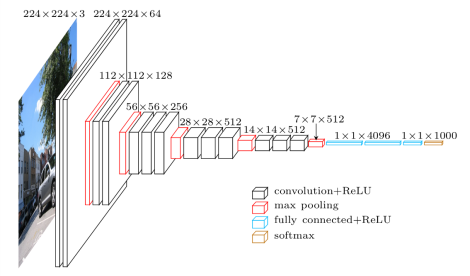
\includegraphics[width=\linewidth]{vgg16}
\caption{Schematic Diagram of VGG16 model}
\label{fig:vgg16schema}
\end{figure}
%
%VGG16 Model
%
%The script for fine--tuning VGG16 can be found in vgg16.py. 
%The first part of the vgg\_std16\_model function is the model schema for VGG16. 
%After defining the fully connected layer, we load the ImageNet pre--trained 
%weight to the model by the following line:

%model.load_weights('cache/vgg16_weights.h5')
%For fine-tuning purpose, we truncate the original softmax layer and replace it with our own by the following snippet:

%model.layers.pop()
%model.outputs = [model.layers[-1].output]
%%model.layers[-1].outbound_nodes = []
%model.add(Dense(num_class, activation='softmax'))
%Where the num\_class variable in the last line represents the number of class labels for our classification task.
%
%Sometimes, we want to freeze the weight for the first few layers so that they 
%remain intact throughout the fine-tuning process. 
%Say we want to freeze the weights for the first 10 layers. 
%%This can be done by the following lines:
%
%%for layer in model.layers[:10]:
%  %  layer.trainable = False
%We then fine-tune the model by minimizing the cross entropy loss function using
%stochastic gradient descent (sgd) algorithm. Notice that we use an initial learning 
%rate of 0.001, which is smaller than the learning rate for training scratch model 
%(usually 0.01).

%sgd = SGD(lr=1e-3, decay=1e-6, momentum=0.9, nesterov=True)
%model.compile(optimizer=sgd, loss='categorical_crossentropy', metrics=['accuracy'])
%model = vgg_std16_model(img_rows, img_cols, channel, num_class)
%Where img_rows, img_cols, and channel define the dimension of the input. For colored image with resolution 224x224, img_rows = img_cols = 224, channel = 3.

%Next, we load our dataset, split it into training and testing sets, and start fine-tuning the model:

%X_train, X_valid, Y_train, Y_valid = load_data()

%model.fit(train_data, test_data,
 %         batch_size=batch_size,
%          nb_epoch=nb_epoch,
 %         shuffle=True,
 %         verbose=1,
  %        validation_data=(X_valid, Y_valid),
 %         )
The fine-tuning process will take a while, depending on your hardware. 
After it is done, we use the model the make prediction on the validation set 
and return the score for the cross entropy loss:

%predictions_valid = model.predict(X_valid, batch_size=batch_size, verbose=1)
%score = log_loss(Y_valid, predictions_valid)


\subsection{Fine-tune Inception--V3}
\label{ssec:inception}
Inception--V3 achieved the second place in the $2015$ \emph{ImageNet} 
competition with a $5.6 \%$ top five error rate on the validation set. 
The model is characterized by the usage of the Inception Module, which is a 
concatenation of features maps generated by kernels of varying dimensions.
%
\begin{figure}[htb]
\centering
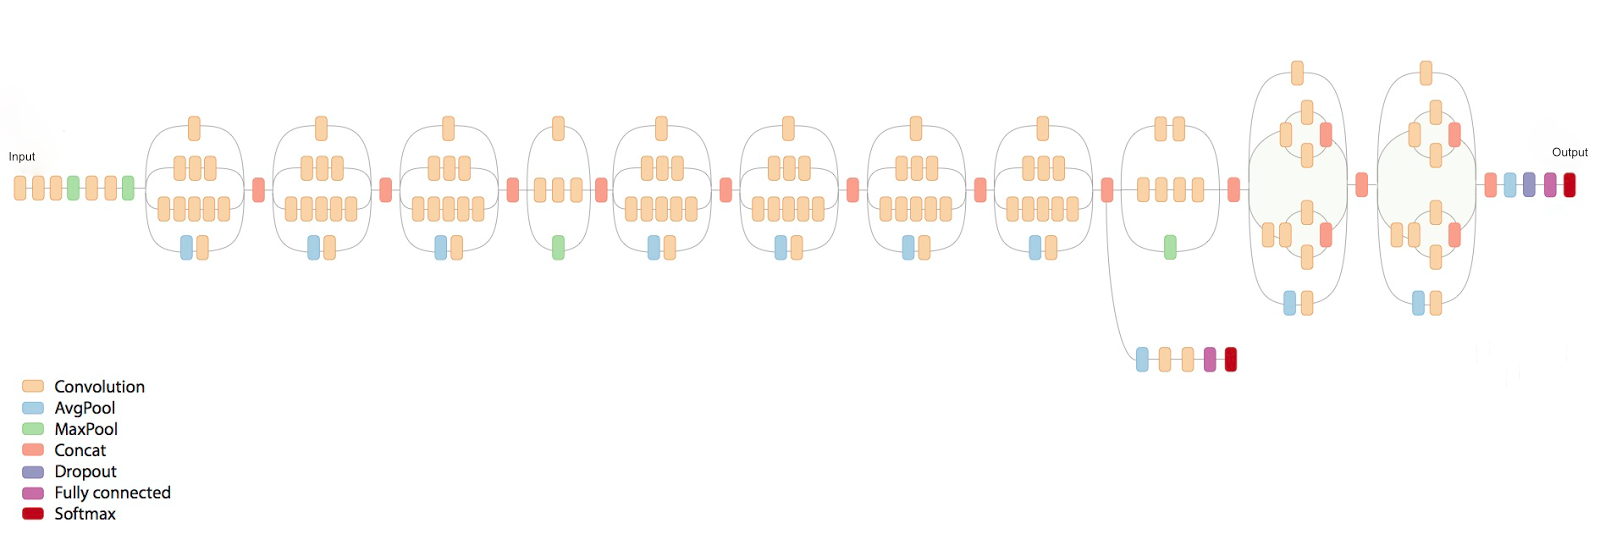
\includegraphics[width=\linewidth]{inception}
\caption{Schematic Diagram of Inception--V3 model}
\label{fig:inceptionV3schema}
\end{figure}
%

%\input{sections/2_section.tex}
	%\subsection{IoT}
%\section{Section 3}
%\label{section3}
%\input{sections/3_section.tex}
%
%\section{Section 4}
%\label{section4}
%%\input{sections/4_section.tex}
%
%%example for Bullet point list
%
%%\begin{itemize}
%%\item example
%%\end {itemize}
%
%
%
%%example for numbered list
%   % \begin{enumerate}
%   % \item example
%
%   % \end{enumerate}
%
%
%
%
%%example for inserting image
%\begin{figure}[h]
%   \centering
%  % \includegraphics[scale=.45]{OWL2}
%    \caption{The structure of OWL2}
%    \label{fig:OWL2}
%\end{figure}
%
%
%%muitextwrite\cite{jj2}.
%
%\section{Conclusion}
%\label {conclusion}
%\input{sections/5_conclusion.tex}
% bibliography
	\bibliographystyle{IEEEtran}
	\bibliography{my-bibliography}
\end{document}
